\documentclass[a4paper]{article}

\usepackage[utf8]{inputenc}
\usepackage[L7x]{fontenc}
\usepackage[lithuanian]{babel}
\usepackage{lmodern}
\usepackage{hyperref}
\usepackage{amsmath} %systems, equations and so on
\usepackage{framed}
\usepackage{graphicx}

\usepackage{geometry}
 \geometry{
 a4paper,
 right=20mm,
 left=20mm,
 top=20mm,
bottom=20mm,
 }

\begin{document}

\makeatletter %creating a special kind of braces
\newenvironment{sqcases}{\matrix@check\sqcases\env@sqcases}{\endarray\right.}
\def\env@sqcases{\let\@ifnextchar\new@ifnextchar \left\lbrack \def\arraystretch{1.2}\array{@{}l@{\quad}l@{}}
}
\makeatother

\section{}

Labas. Su jumis kalba patsai \href{run:portretas.jpg}{\textbf{Saimonas!}}
\section{}
Paspauskite mano vardą. Ar mane matote? Išnagrinėsime visus galimus atvejus:

$\begin{sqcases}
\text {Mane matote} \Rightarrow \text{jums \href{http://www.soundjay.com/human/sounds/applause-01.mp3}{\textbf{ploju}}} \\
\text {Manęs nematote} \Rightarrow 
\begin{sqcases}
\text {Nenorite matyti} \Rightarrow \text{Išjunkite kompiuterį ir išeikite pakvėpuoti grynu oru} \\
\text {Norite matyti} \Rightarrow \text{Atsidarykite šį failą per \href{https://get.adobe.com/reader/}{\textbf{Acrobat Reader}}}
\end{sqcases}
\end{sqcases}$

\section{}

Būna, kai Saimonui gera nuotaika, jis pasakoja istorijas.

\begin{framed}
\textit{Berniukai reikalauja laiko ir pinigų:} 

$BOYS=TIME \cdot MONEY$

\textit{Laikas ir yra pinigai, todėl}

$BOYS=MONEY \cdot MONEY=MONEY^2$

\textit{Pinigai yra blogio šaknis, todėl }

$BOYS=\Big(\sqrt{EVIL}\Big)^2=EVIL$
\end{framed}

Tačiau kartais jos yra panašios į kažkokį briedą. \href{mailto:simonas.mamaitis@gmail.com}{\textbf{Pasakykite}}, kas čia ne taip.

\section{}

Būna, kai Saimonui bloga nuotaika, jis atrodo \href{https://www.facebook.com/photo.php?fbid=1791779717765839&set=a.1720498398227305.1073741828.100008014839713&type=3&theater}{\textbf{ne kaip}}

\section{}

Saimonas nėra vienišas. Jis turi draugių, pavyzdžiui \href{http://pastebin.com/ASmJ06mu}{\textbf{Dianą}}, \href{http://pastebin.com/yqhNy1UR}{\textbf{Karoliną}} ir \href{http://pastebin.com/xKmSuHfM}{\textbf{Grėtę}}.

\section{}

Kai Saimonas užsiima muzika, jis kuria \href{https://soundcloud.com/naktinis-saimonas/simon-production}{\textbf{garsą}} iš matematikos formulių.

\section{}

Kai Saimonas užsiima matematika, jis rašo sudėtingą matematikos \href{run:diskr.pdf}{\textbf{konspektą}} iš daug raidžių.

\section{}

\href{http://www.youtube.com/watch?v=7WwLT32_VAk&t=23m30s}{\textbf{Likit sveiki!}}

\begin{center}
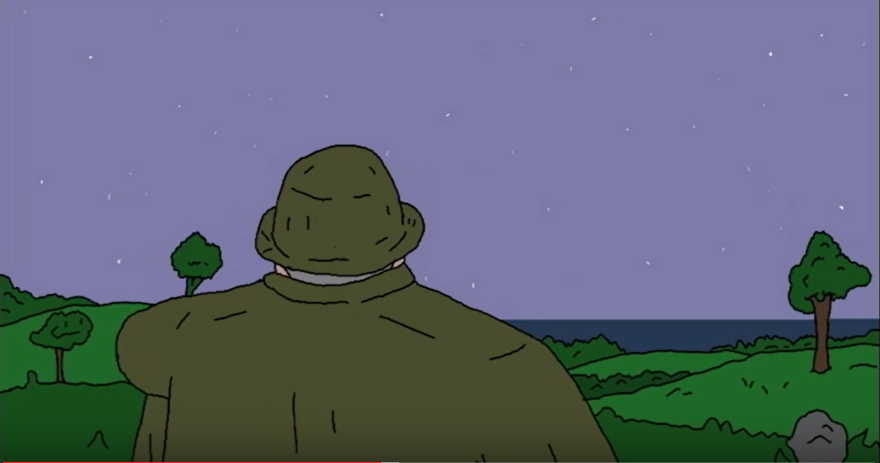
\includegraphics[width=80mm]{fairy.png}
\end{center}
\end{document}